\documentclass{article}
\usepackage{hyperref}
\usepackage{graphicx}
\usepackage{xcolor}

\title{MapReduce on GPU}
\author{Mark Doughten [md1875], \\ Abhilash Nambissan [ajn125], \\ Rishita Mane [rm1848]}
\date{April 27, 2025}

\begin{document}

\maketitle

% \section{Links to project}
Project Github link: https://github.com/markdoughten/mapreduce


\section{Introduction}
The MapReduce framework was originally designed at Google for processing  parallelizable problems on large datasets, by distributing work across many nodes. \cite{mapreduce}. Given that commodity GPUs today contain hundreds or even thousands of processing cores, it is an interesting avenue of research to utilize this massive parallel processing capability for map-reduce style processing jobs. Some prior works exist in this area, notably Mars \cite{mars}, one of the major attempts at providing a MapReduce programming framework for the GPU programming interface. In our project we aim to analyse the performance of Mars, identify some of the performance issues that exist, and implement our own variant of GPU MapReduce which addresses some the identified issues. We evaluate our version by comparing its performance to Mars's performance on the same workloads. 

\section{Prior Work}
\subsection{MapReduce}
MapReduce is a programming model developed initially at Google, for processing very large data sets. This model splits the work into smaller jobs, and executes the jobs in parallel on a cluster of worker nodes, finally aggregating the results of the jobs into the final results. Various parallel and distributed algorithms are used for the batch processing as well as aggregation of partial results. A typical MapReduce application involves four main stages:
 \begin{enumerate}
     \item Input Splitting: In this stage, the system divides the input data into small chunks, and each chunk is assigned to one Map worker. The splits are typically generated in the form of key-value pairs.
     \item Map procedure: The Map function reads a series of input key-value pairs, performs some computation on them, and generates a series of output key/value pairs. The types of the input and output key-value pairs can be (and usually are) different from each other.
     \item Grouping intermediate output: The system takes the key-value pairs generated by the Map stage, and groups the pairs which have the same key. This requires sorting the key-value pairs generated across all Map worker nodes, so that all pairs with the same key are next to each other in the final sorted order. The sorting is usually done using some parallel sorting algorithm.
     \item Reduce procedure: The Reduce function takes the group of all key-value pairs corresponding to a particular key, and aggregates all the values in that group into a single output, which is usually the key itself and one value representing the aggregate of all values for that key.
 \end{enumerate}

\begin{figure}[ht]
    \centering
    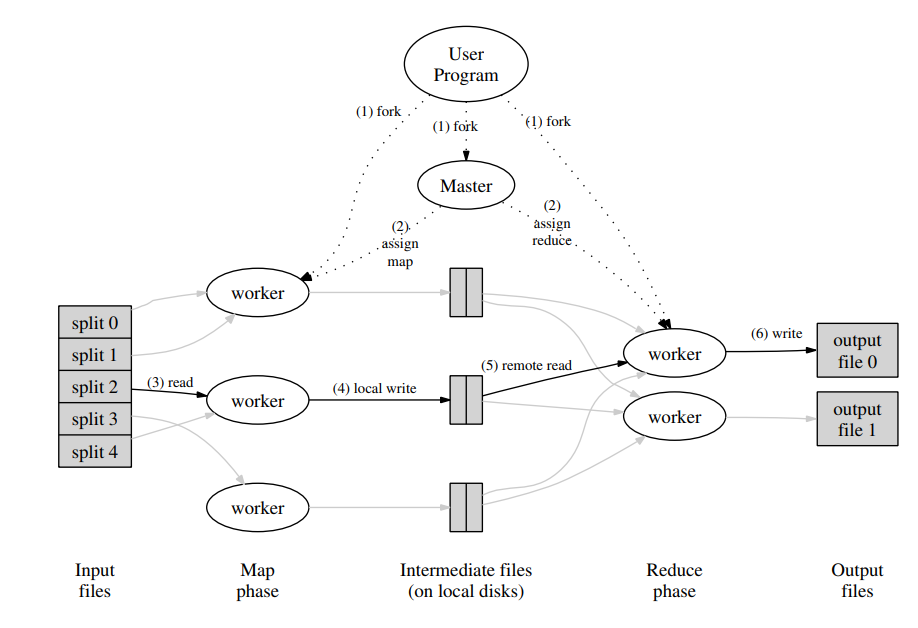
\includegraphics[width=1\linewidth]{./images/mapreduce.png}
    \caption{MapReduce Framework \cite{mapreduce}}
    \label{fig:mapreduce}
\end{figure}

The MapReduce model assigns work to worker nodes (map workers and reduce workers). While Google's (and many other) implementation of the MapReduce model used a cluster of machines, where each machine is considered as an individual node, the MapReduce model can technically be applied to any granularity of parallel processing capability. For example, the individual cores on a single machine's multi-core processor can be considered
as individual nodes. For GPUs which have hundreds of processing cores, each core can be considered as an individual node which can do work in parallel with others. 

\subsection{Mars: A MapReduce Framework on Graphics Processors}
Mars was a research project that developed a Map Reduce implementation that takes advantage of GPU processing capabilities. Although GPU programming frameworks like CUDA exist, it requires significant expertise to implement a MapReduce-style processing pipeline in such frameworks. The major goals of the Mars project were to provide a developer friendly programming framework, built on top of CUDA, to allow developers to more easily express their application logic in a MapReduce way, which can then be executed on the GPU. Additionally, providing performance equal to or better than comparable CPU implementations was also a major goal. The evaluation of their implementation in their research paper shows that they were able to meet these goals on hardware available at the time. 


\section{Project Goals}
\subsection{Motivation}
We performed some performance and scalability analysis on the Mars framework, and identified several opportunities for improvement. We specifically profiled their implementation for the Word Count use-case, and found the following issues. 
\begin{enumerate}
    \item Inefficient algorithmic techniques: We observe that the amount of time taken to running relatively small datasets (by present standards) is not in line with what is expected from the performance capabilities of current GPU hardware. A detailed profiling of the executed CUDA code shows that a massive amount of time is taken in the Sorting and Grouping stage, as much as 85\%-90\% of the overall run time of the application. A deeper look at the actual algorithms used in Mars for performing sorting and grouping indicate that there is ample opportunity for improvement.
    \item Inefficient GPU resource usage: From the profiling data, we also see that the resource consumption (specifically memory usage) when the GPU code is running seems to be very high, compared to what would be expected based on a rough calculation of how much memory would be needed to do what the framework does. We identified two major causes for this: use of inefficient data structures to hold various stages of intermediate data, and not freeing intermediate data when they are no longer required for further computations. 
    \item Scalability problems: Further to the previous point, we observe that the peak GPU memory usage is as high as 4x-5x the size of the original input. Considering that commodity consumer-grade GPUs of today only have about 8-16GB of memory on average, this severely limits the size of data that can be processed using this framework. 
\end{enumerate}

\subsection{Goals}
Based on the areas of improvement identified as mentioned above, our goal is design an enhanced version of GPU-based MapReduce which addresses these issues. The main design goals of our implementation are:
\begin{enumerate}
    \item Achieve significant performance speed up in the overall computation time by using better algorithms for the various stages
    \item Achieve significant reduction in GPU memory consumption by using more efficient ways of storing intermediate data, as well as better memory management in terms of efficient allocation and freeing.
    \item Use the above two improvements to improve the scalability of the framework, i.e. gracefully handling larger data sizes compared to what Mars is capable of, on the same hardware.
\end{enumerate}




\section{Design}
In this section we first present a brief summary of some key design aspects of Mars, with a focus on the WordCount application specifically. Later we describe how our implementation differs from the former.

\subsection{Mars design summary} \label{mars-design-summary}
The Mars framework operates in 8 main stages. 
\begin{enumerate}
    \item Read \& preprocess input: Read the input from the specified file and perform any required preprocessing on it. In the case of the Word Count application, the preprocessing involves converting all alphabets in the input text to uppercase. 
    \item Split file blocks: Split the preprocessed text from the file into small blocks. For WordCount, this involves splitting the text into chunks of 2048 characters on average. It also makes sure that a split doesn't happen in the middle of a word, some some chunks might be slightly larger or smaller than 2048 characters.
    \item Pre-compute map output size: Run a CUDA kernel to calculate total output size for all the key-value pairs that each CUDA thread will generate. Not that this step does not actually emit the key-value pairs, only the size (in bytes) that would be needed to store the key-value pairs. 
    \item Allocate GPU memory for Map output: Step 3 gives the total size of memory that needs to be allocated in the GPU to hold all key-value pairs from all threads. 
    \item Pre-compute per-thread memory offsets: Since we already know exactly how much memory each thread is going to use in advance, each thread can now write to a particular contiguous chunk of the allocated memory. This will prevent multiple threads from attempting to write in the same memory locations, which significantly improves thread performance in CUDA. A CUDA kernel which does a prefix-sum is run on the per-thread output size array from step 3, which gives an array of starting offsets in the memory buffer from where each thread can begin writing. 
    \item Map operation: Run a CUDA kernel where every thread executes the Map function specified. For WordCount, every thread goes through the block of text allocated to it, parses words in the text and assigns a count of '1' for every word.
    \item Sort/Group operation: All the key value pairs are sorted based on the key. A version of the 'bitonic sort' parallel sorting algorithm is implemented in the Mars framework to perform the sorting.
    \item Combine/Reduce: Using the sorted key-value pairs, combine the count values for all key-value pairs with the same key.
\end{enumerate}


\subsection{Our design improvements}
\subsubsection{Efficient pre-computation of output memory offsets}
For the computation of offsets in stage 5 (refer section \ref{mars-design-summary}), Mars uses a self-implemented prefix-sum based approach. This approach allocates a new array in GPU memory to hold the prefix sums at each index.

In contrast, we use a proven high-performance CUDA version of prefix-sum, included in the Nvidia "Thrust" library, which has recently become a part of the CUDA standard library. This version is expected to be more performant, and also notably, it performs the prefix sum in-place. We identify that none of the future stages actually need the original output of stage 3, all future stages after stage 5 can work with just the prefix sum output. So performing the prefix-sum in-place does not destroy any necessary information, while at the same time enabling us to avoid additional memory overhead for storing the output.

\subsubsection{Efficient use of memory for storing intermediate data and metadata} \label{efficient-metadata}
We observe that for Word Count, and many similar MapReduce applications, the value for every key-value pair initially generated by the map stage is a constant value. For example, for Word Count, every key-value pair has a value of 1 when initially generated in the Map function. The Mars framework allocates an array of integers for every key-value pair produced, just to store the value 1 in every element of the array. Given a large input data set which will generate millions of key-value pairs, this is significantly inefficient and could potentially be avoided. 

In our design, we identify another possible optimization: we use the value in each key-value pair to store the offset location of the corresponding key (word) in the original input buffer. Storing this metadata helps us to make subsequent operations in the later stages more efficient, as we will describe in the following sections. 

// INSERT IMAGE OF KEY AND VALUE ARRAYS HERE

\subsubsection{Improved method for sorting intermediate key-value pairs}
The sorting algorithm implemented in Mars uses a custom implementation of the "bitonic sort" algorithm for performing parallel sort. Upon inspecting the code for this implementation, we see that it involves repeated usage of their own prefix-sum kernel, as well as significant copying and moving around of the key strings in GPU memory using a self-implemented GPU string processing library.  This could potentially cause slow performance of the sorting algorithm, and also cause significantly high memory usage. Our profiling data shows both of these to be true.

//INSERT PROFILING OF MARS FIGURE HERE

We implement a different way of sorting in our design, by utilizing the offsets we store in the key-value pairs in the Map stage, as mentioned in section \ref{efficient-metadata}. Refer to the figure which shows the layout of the keys and values in memory. We perform the sort only on the values array, i.e the offset values, based on the alphabetical order of the keys which begin at those offsets. This helps us to perform in place sorting on just an array of integers, while not moving any of the strings in the Keys array. Additionally, we also use a proven high-performance implementation of parallel sort, again from the Nvidia "Thrust" library.  We run this sort method on the values array, while providing a custom comparison operator which actually compares the corresponding strings in the Keys array, rather than the offset values themselves. Since we never perform any operations on the actual strings, we entirely avoid the need for any kind of string processing library.

This implementation shows significantly better performance and significantly lower memory usage (details to follow in the Evaluation section).

// INSERT BEFORE AND AFTER SORT IMAGES HERE


\subsubsection{Improved method to combine final values}
Mars uses a custom implementation to go through the sorted key-value pairs for de-duplication and combining. In contrast, we utilize our sorted metadata offsets in conjunction with a standard reduce operator provided in the Nvidia Thrust library. We run the reducer by using the offset values as keys, rather than the word strings. As before, we provide a custom comparison operator to the reducer which will actually perform the comparison based on the strings in the Keys array, rather than the offsets themselves.


\subsubsection{Improved memory allocation and freeing}
Referring back to the stages in \ref{mars-design-summary}, we identified a few points in the execution where some intermediate data is no longer needed in any of the future stages. Most notably, we identify that after the key-value pairs have been generated in the Map operation, we no longer need to keep the original text file data in GPU memory, as well as the initial key-value pairs indicating the splits. We remove these data from GPU memory as soon as the Map stage is done, which enables to significantly reduce the peak memory usage of our implementation.

// INSERT BEFORE AND AFTER REDUCE IMAGES HERE

\section{Evaluation}
We compare our version of GPU MapReduce with the Mars version. We run the Word Count implementation provided in the Mars repository, and compare it against our implementation which is also focused on Word Count. We run a variety of data sizes and compare various performance metrics, such as total run time, run time for individual stage CUDA kernels, memory usage, etc.

\subsection{Workload: Word Count}
The Word Count use-case involves reading a large amount of text data, and counting the frequency of appearance of each word in the body of text. The input is a text file which contains the text. The output is a list of key value-pairs, where the key is a unique word, and the corresponding value is the number of times that word appears in the given text file. We run various sizes of text files including 256MB, 512MB, 1GB, 1.5GB, 2GB and 3GB. The text of the required size is generated by repeatedly duplicating the text of the novel "Frankenstein" by Mary Shelley, sourced from Project Gutenberg.  

\subsection{Evaluation setup}
Our experiments are performed on a recent commodity laptop with the following specifications:
\begin{itemize}
    \item Processor: 
    \begin{itemize}
       \item AMD Ryzen 7 7745HX single-socket processor (Zen 4 architecture)
       \item 8 cores, 16 threads @ 3.1 GHz
       \item 16GB
    \end{itemize}
    \item GPU: Nvidia RTX 4070 Max-Q Mobile (Ada Lovelace architecture)
    \begin{itemize}
        \item 4608 CUDA cores @ 1.61 - 2.8 GHz
        \item 8GB GDDR6 memory
        \item 128KB per-cluster L1 cache, 32MB shared L2 cache
    \end{itemize}
    \item Memory: 16GB DDR5 memory
    \item Software:
    \begin{itemize}
        \item OS: Ubuntu 24.04
        \item NVIDIA Driver version: 570.133.20
        \item CUDA version: 12.8
        \item Profiling tools: NVIDIA NSight Systems 2025
    \end{itemize}
\end{itemize}

\section{Results}
\subsection{Overall performance}
We measure the overall performance in terms of total run time of the application, on various data sizes. The following graph shows the observed data. From the graph, we can clearly see that our implementation completes significantly faster than the Mars version. Further, we also see that the margin of difference increases with increasing sizes of input. This indicates that our version is both more performant, and has better scalability than 
the Mars version.

// INSERT RUNTIME COMPARISON FIGURE HERE

\subsection{CUDA Kernel analysis}
We used the NVIDIA NSight profiler to gain deeper insight into the execution of the different CUDA kernels in the various stages of the applications. Figures x and y show the CUDA kernel profile for Mars and our version respectively. We can see that in Mars, a huge amount of time is spent on the bitonic sort kernels. Also, the time for the sort increases significantly when the input size is increased. In contrast, we see that out version spends relatively a much smaller amount of time performing the sort operations. Also, the rate of increase for sorting time, when increasing input sizes, is much smaller.

// INSERT PROFILES AND COMPARISON GRAPHS HERE

This can be explained by two main factors:
\begin{enumerate}
    \item Sorting on integers, with no movement of strings: This aspect of our design reduces the amount of data copy operations involved in the sorting.
    \item Using better parallel implementations: The data clearly shows that the merge sort technique used by the Thrust library performs much better than Mars's bitonic sort implementation. Existing research work indicates that the algorithm used in Thrust performs better than basic bitonic sort, particularly for large inputs. Additionally the Thrust library has been continuously improved and optimized for a decade, so it can be expected that it performs better than a custom implementation from the time period when Mars was implemented.
\end{enumerate}


\subsection{Memory usage}
We used the profiler to visualize the GPU memory usage of the application throughout its run time. Figures x and y show the memory usage trend for Mars and our version respectively, for a 1GB input text file. We can see that the memory usage for Mars is as high as 5GB (5x the size of the original input), whereas our design uses only a maximum of 2GB throughout the run. 

// INSERT PROFILES AND COMPARISON GRAPHS HERE

This can be explained by a combination of factors:
\begin{enumerate}
    \item We avoid storing redundant data in memory ref:\ref{} 
    \item We perform operations like prefix-sum in-place, rather than generating copies ref:\ref{}
    \item We do not allocate additional memory for copying key strings during sorting and reducing ref:\ref{}
    \item We free data from GPU memory as soon as it is certain that it will not be needed in the future. ref:\ref{}
\end{enumerate}


\subsection{Scalability analysis}
We try running both versions with larger data sets, up to 3GB in size. We see that on our machine's GPU which has 8GB of memory, Mars runs out of memory for file sizes starting from 1.5GB. Whereas, our version can comfortably run file sizes as large as 3GB. This is due to the lower overall and peak memory used by our implementation, as compared to Mars.



\section{Conclusion}
GPUs with thousands of processing cores are a very promising platform for running MapReduce-style parallel processing jobs, even on consumer-grade hardware. However, as of today, given the relatively complex GPU programming model, as well as relatively smaller size of on-board GPU memory, MapReduce programs must be written with careful focus on performance optimization in order to get the best possible utilization of the GPU hardware and software capabilities. 
In this work, we have analyzed the design and performance characteristics of a prior MapReduce implementation for GPUs, and identified areas of improvement. We have implemented a modified design which focuses on three key forms of optimization:
\begin{enumerate}
    \item Efficient usage of available memory to store only relevant and useful data.
    \item Performing expensive operations such as sorting, grouping, etc. on integer indices representing the string keys, rather than on the strings themselves.
    \item Utilization of battle-tested high-performance libraries for expensive operations, taking advantage of the last 15 years of research and progress in GPU computing techniques.
\end{enumerate}

Our evaluations show that our version performs significantly better than the previous implementation, up to a factor of 2x-5x. The performance improvement is observed in terms of application run time, memory movement and memory usage, and all these factors make our design significantly more scalable as well. 

\begin{thebibliography}
\raggedright

\bibitem{mapreduce}
J. Dean and S. Ghemawat, \textit{MapReduce: Simplified Data Processing on Large Clusters}. \href{https://dl.acm.org/doi/10.1145/1327452.1327492}{https://dl.acm.org/doi/10.1145/1327452.1327492}

\bibitem{mars}
B. He, W. Fang, Q. Luo, N. Govindaraju, and T. Wang, \textit{Mars: A MapReduce Framework on Graphics Processors}. \href{https://dl.acm.org/doi/10.1145/1454115.1454152}{https://dl.acm.org/doi/10.1145/1454115.1454152}

\bibitem{cuda_docs}
NVIDIA, \textit{CUDA C Programming Guide}. \href{https://docs.nvidia.com/cuda/cuda-c-programming-guide/contents.html}{https://docs.nvidia.com/cuda/cuda-c-programming-guide/contents.html}

\bibitem{cuda_mem_pool}
NVIDIA, \textit{CUDA Memory Pools API}. \href{https://docs.nvidia.com/cuda/cuda-runtime-api/group__CUDART__MEMORY__POOLS.html}{https://docs.nvidia.com/cuda/cuda-runtime-api/group\_\_CUDART\_\_MEMORY\_\_POOLS.html}

\bibitem{cuda_forum_async}
NVIDIA Developer Forum, \textit{Confusion about Synchronization and cudaMemcpyAsync}. \href{https://forums.developer.nvidia.com/t/confusion-about-synchronization-or-asynchronization-of-cudamemcpy-and-cudamemcpyasync/276826/4}{https://forums.developer.nvidia.com/t/confusion-about-synchronization-or-asynchronization-of-cudamemcpy-and-cudamemcpyasync/276826/4}

\bibitem{dynamic_scheduling}
M. Steinberger, \textit{On Dynamic Scheduling for GPUs}. \href{https://www.markussteinberger.net/papers/OnDynamicScheduling.pdf}{https://www.markussteinberger.net/papers/OnDynamicScheduling.pdf}

\bibitem{pinned_memory}
A guide on good usage of non\_blocking and pin\_memory() in PyTorch. \href{https://pytorch.org/tutorials/intermediate/pinmem_nonblock.html}{https://pytorch.org/tutorials/intermediate/pinmem\_nonblock.html}


\end{thebibliography}

\end{document}